\documentclass[11pt]{article}

% Biên dịch bằng XeLaTeX hoặc LuaLaTeX để hiển thị tiếng Việt đầy đủ.
\usepackage{fontspec}
\setmainfont{lmroman10-regular.otf}[
  Path=/usr/local/texlive/2026basic/texmf-dist/fonts/opentype/public/lm/,
  BoldFont=lmroman10-bold.otf,
  ItalicFont=lmroman10-italic.otf,
  BoldItalicFont=lmroman10-bolditalic.otf
]
\usepackage[margin=1in]{geometry}
\usepackage{graphicx,booktabs,longtable,array,amsmath,amssymb,xcolor}
\usepackage[colorlinks=true,linkcolor=blue,citecolor=blue,urlcolor=blue]{hyperref}
\usepackage{caption,float,enumitem,fancyhdr,titlesec,pifont}
\usepackage{url}
\urlstyle{tt}
\renewcommand{\UrlFont}{\ttfamily\small}
\Urlmuskip=0mu plus 1mu

\definecolor{navy}{HTML}{0B132B}
\definecolor{slate}{HTML}{64748B}
\newenvironment{luuy}[1][Lưu ý]
  {\begin{quote}\small\color{slate}\textbf{#1.}\ }
  {\end{quote}}
\titleformat{\section}{\normalfont\Large\bfseries\color{navy}}{\thesection}{1em}{}
\titleformat{\subsection}{\normalfont\large\bfseries\color{navy}}{\thesubsection}{1em}{}
\pagestyle{fancy}\fancyhf{}
\fancyhead[L]{\small\color{slate}AI Race: tổng hợp thí điểm đa mô hình}
\fancyhead[R]{\small\color{slate}\thepage}
\renewcommand{\headrulewidth}{0.4pt}
\setlength{\headheight}{13pt}

\title{\textbf{Hành vi của các mô hình ngôn ngữ trong trò chơi ``AI Race''}\\[0.3em]
\large Báo cáo thí điểm: so sánh mô hình, số người chơi và dữ liệu con người}
\author{AI Race Experiment --- Cross-Model Pilot Synthesis}
\date{\today}

\begin{document}
\maketitle

\begin{abstract}
Báo cáo này so sánh cách con người và năm phiên bản mô hình ngôn ngữ lớn (LLM)
chơi trò chơi lặp lại ``AI Race''. Mỗi lượt, người chơi chọn \textsc{An toàn}
hoặc \textsc{Mạo hiểm}. Mạo hiểm giúp tiến nhanh và kiếm nhiều hơn ngay lúc đó,
nhưng có thể dẫn đến mất toàn bộ phần thưởng nếu người chơi về đích trước hoặc
hòa. Chúng tôi dùng dữ liệu của 341 người tham gia và các lượt chơi của GPT-5
nano, GPT-5.4 nano, Gemini 3 Flash, Gemini 3.1 Flash Lite và Gemini 3.5 Flash
Lite; một phần thí nghiệm mở rộng có 3--5 người chơi.

Kết quả chính là: không có mô hình nào có hành vi giống toàn bộ nhóm người, và
các mô hình cũng khác nhau rõ rệt. Nhãn vai trò hoặc cách diễn đạt về mức chấp
nhận rủi ro ảnh hưởng đến lựa chọn mạnh hơn bản thân mức rủi ro trong luật chơi.
Tuy vậy, đây chỉ là dữ liệu thí điểm: các kết quả là mô tả và gợi ý để kiểm tra
tiếp, không phải bằng chứng khẳng định cuối cùng.
\end{abstract}

\tableofcontents
\clearpage

\section{Bài toán, dữ liệu và cách đọc báo cáo}

\subsection{Trò chơi AI Race}
Trong mỗi lượt, các đối thủ chọn đồng thời một trong hai hành động. Chọn
\textsc{An toàn} cho tiến độ ổn định. Chọn \textsc{Mạo hiểm} cho tiến độ và
điểm của lượt đó cao hơn, nhưng làm tăng nguy cơ bị ``thụt lùi''. Nguy cơ này
chỉ được xét khi người chơi thắng hoặc hòa cuộc đua; khi xảy ra, toàn bộ phần
thưởng tích lũy có thể bị xóa. Trò chơi có ít nhất 5 lượt; sau đó, mỗi lượt có
20\% khả năng kết thúc. Vì thế không ai biết trước lượt nào là lượt cuối.

Ba điều cần phân biệt trong báo cáo là: (i) \emph{mức rủi ro} trong luật chơi,
có giá trị tối đa 0.1, 0.6 hoặc 0.9; (ii) \emph{tỷ lệ chọn Mạo hiểm}, tức phần
trăm lượt mà một người chơi chọn hành động này; và (iii) \emph{nhãn vai trò},
ví dụ R1 là cách mô tả khuyến khích thận trọng nhất còn R6 là cách mô tả
khuyến khích chấp nhận rủi ro nhất. Nhãn vai trò không thay đổi luật chơi.

\subsection{Dữ liệu}
\begin{table}[H]\centering\small
\begin{tabular}{@{}p{3.9cm}p{2.9cm}p{1.8cm}p{5.8cm}@{}}\toprule
\textbf{Nguồn} & \textbf{Nhóm} & \textbf{Quy mô} & \textbf{Nội dung}\\\midrule
\url{references/human_data/} & 341 người & 3.245 dòng lượt chơi & Dữ liệu đã khử định danh của nghiên cứu gốc.\\
\url{results/frontier/} & 5 LLM, 2 người chơi & 20--50 người chơi/mức rủi ro/mô hình & Điều kiện trung tính và các điều kiện gán vai trò.\\
\url{results/nplayer/openai/} & GPT-5 nano, GPT-5.4 nano & 3--5 người chơi & Điều kiện trung tính, vai trò R1--R6 và phối hợp vai trò đối đầu/hợp tác.\\
\bottomrule\end{tabular}
\caption{Các nguồn dữ liệu được dùng. Không gộp dữ liệu giữa mô hình, giữa trò chơi 2 người và nhiều người, hoặc giữa người và LLM.}
\label{tab:data-sources}\end{table}

Các thư mục chạy được kiểm tra lại bằng cách đối chiếu số lượt và số ván khai
báo với tệp ghi kết quả. Trong dữ liệu 2 người chơi, 121/137 thư mục đạt yêu
cầu; 16 thư mục lỗi, đang chạy dở hoặc có nhật ký bị lặp bị loại. Toàn bộ 41
thư mục thí nghiệm nhiều người chơi đạt yêu cầu; hơn 22.000 quyết định được đọc
mà không có lỗi phân tích.

\begin{luuy}[Sửa lại một ghi nhận về chất lượng dữ liệu]
Một thư mục Gemini 3 Flash từng bị mô tả nhầm là nhật ký trùng hoàn toàn với 15
ván chuẩn. Kiểm tra đủ 15 ván cho thấy chỉ các ván ở mức rủi ro 0.1 giống hệt;
ở mức 0.6 và 0.9, chuỗi hành động khác nhau. Đây là một lần chạy lại độc lập
nhưng dùng chung hạt ngẫu nhiên của ván. Thư mục vẫn bị loại vì ghép nó vào sẽ
làm các quan sát không còn độc lập như giả định của phân tích, chứ không phải vì
nó là bản sao. Sửa này chỉ đổi các con số liên quan 1--2 điểm phần trăm và không
đổi kết luận nào.
\end{luuy}

\subsection{Các giả thuyết được kiểm tra}
Để tránh để kết quả xuất hiện mà không có câu hỏi dẫn đường, báo cáo dùng bảy
giả thuyết sau. Mỗi phần sẽ nêu rõ dữ liệu, kết quả và mức độ chắc chắn.
\begin{enumerate}[leftmargin=*]
\item \textbf{H1 -- Các mô hình phản ứng giống nhau trước mức rủi ro.} Nếu đúng,
đường tỷ lệ chọn Mạo hiểm theo ba mức rủi ro sẽ có hình dạng tương tự.
\item \textbf{H2 -- Rủi ro trong luật chơi quan trọng hơn cách gán vai trò.} Nếu
đúng, thay đổi mức rủi ro sẽ làm hành vi đổi nhiều hơn đổi R1--R6.
\item \textbf{H3 -- LLM tái tạo các quy luật động của con người.} Quy luật động
là phản ứng với hành động lượt trước của đối thủ và vị thế đang dẫn hay tụt.
\item \textbf{H4 -- Những yếu tố dự báo lựa chọn Mạo hiểm giống nhau ở người và
LLM.}
\item \textbf{H5 -- Tăng số người chơi không làm thay đổi kiểu hành vi cốt lõi.}
\item \textbf{H6 -- Chọn Mạo hiểm nhiều hơn luôn đem lại lợi ích thực tế.}
\item \textbf{H7 -- Các mô hình gần dự đoán lý thuyết hơn cũng giống con người
hơn.}
\end{enumerate}

\subsection{Phương pháp, nói ngắn gọn}
Chúng tôi dùng hồi quy logistic để xem một yếu tố có liên quan với xác suất
chọn Mạo hiểm hay không; mô hình được tính sai số theo từng khối ván dùng chung
ngẫu nhiên. Rừng ngẫu nhiên và SHAP được dùng để xếp hạng các biến giúp dự báo
lựa chọn; đây là công cụ mô tả, không chứng minh nguyên nhân. Phân cụm $k$-means
gom những người có mẫu hành vi gần nhau. Khi so sánh hai mô hình thống kê lồng
nhau, kiểm định tỷ số hợp lý (LR) trả lời liệu mô hình phức tạp hơn có giải
thích dữ liệu tốt hơn đáng kể hay không.

Mọi hình và bảng có thể tái tạo từ các mã trong \texttt{results/scripts/};
số liệu gốc được lưu dạng bảng máy đọc được trong \texttt{data/}.

\clearpage
\section{H1: Các mô hình có phản ứng giống nhau trước rủi ro không?}
\label{sec:heterogeneity}

\textbf{Giả thuyết H1.} Nếu các mô hình có cùng cách phản ứng trước rủi ro,
đường tỷ lệ chọn Mạo hiểm theo các mức 0.1, 0.6 và 0.9 sẽ gần giống nhau.
\textbf{Kết luận: bác bỏ H1 trong dữ liệu thí điểm.} Các mô hình không chỉ khác
về mức trung bình mà còn khác về hình dạng phản ứng.

GPT-5 nano gần như luôn chọn An toàn (chỉ 6--9\% lượt là Mạo hiểm). GPT-5.4
nano ở mức trung bình (51--55\%). Ba mô hình Gemini gần như luôn Mạo hiểm ở
mức rủi ro 0.1 rồi giảm khi mức trần rủi ro tăng. Hướng giảm này giống hướng
trong dữ liệu người, nhưng độ thay đổi lớn hơn 4--15 lần.

\begin{figure}[H]\centering

\includegraphics[width=.92\linewidth]{figures/cross_model_risk_response_neutral.png}
\caption{Tỷ lệ Mạo hiểm trung bình của từng mô hình theo mức trần rủi ro, ở điều kiện không gán vai trò. Vùng tô là khoảng tỷ lệ của nhóm người.}
\label{fig:risk-response}\end{figure}

Kiểm định LR trên 4.464 quyết định cho thấy: cho phép mỗi mô hình có đường phản
ứng rủi ro riêng cải thiện mạnh so với việc chỉ cho chúng khác nhau về mức
trung bình (LR = 354,7; 10 bậc tự do; $p=4\times10^{-70}$). Nói đơn giản, khác
biệt này khó có thể chỉ do nhiễu ngẫu nhiên.

\begin{luuy}
Một vài ô dữ liệu có hành vi gần 0\% hoặc 100\%, làm phép ước lượng có cảnh báo
số học. Vì vậy con số LR chính xác chỉ nên xem là xấp xỉ; kết luận định tính
rằng các đường phản ứng khác nhau vẫn rất rõ.
\end{luuy}

\subsection{So với con người}
Không mô hình nào tái tạo đầy đủ tám dấu hiệu từ nghiên cứu trên người. GPT-5
nano thấp hơn nhiều so với người. GPT-5.4 nano có tỷ lệ trung bình nằm trong
khoảng của người, nhưng các phản ứng theo lịch sử lượt chơi không cùng hướng.
Các Gemini Lite tái tạo được hướng thay đổi theo rủi ro và hầu như không có
người chơi luôn An toàn, nhưng tỷ lệ Mạo hiểm nói chung lại quá cao.

\begin{table}[H]\centering\small
\begin{tabular}{@{}lcccccccc@{}}\toprule
\textbf{Mô hình} & E1 & E2 & E3 & E4 & E5 & E6 & E7 & E8\\\midrule
GPT-5 nano & ? & ? & ? & ? & \ding{55} & \ding{55} & \ding{55} & \ding{55}\\
GPT-5.4 nano & \ding{55} & \ding{55} & \ding{55} & \ding{55} & \checkmark & \checkmark & \checkmark & \ding{55}\\
Gemini 3 Flash & ? & ? & ? & ? & \ding{55} & \checkmark & \ding{55} & \checkmark\\
Gemini 3.1 Flash Lite & ? & ? & ? & ? & \ding{55} & \checkmark & \ding{55} & \checkmark\\
Gemini 3.5 Flash Lite & ? & ? & ? & ? & \ding{55} & \checkmark & \checkmark & \checkmark\\
\bottomrule\end{tabular}
\caption{Bảng đối chiếu tám dấu hiệu của nghiên cứu trên người. E1: hành động trước của đối thủ; E2: chênh tiến độ; E3: hành động lượt đầu; E4: hành động trước của bản thân (ở người không có hiệu ứng); E5: so sánh rủi ro 0.6 với 0.9 (ở người không có hiệu ứng); E6: so sánh 0.1 với 0.6; E7: tỷ lệ Mạo hiểm chung; E8: tỷ lệ luôn An toàn. Dấu hỏi nghĩa là không thể ước lượng ổn định.}
\label{tab:scorecard}\end{table}

\begin{figure}[H]\centering
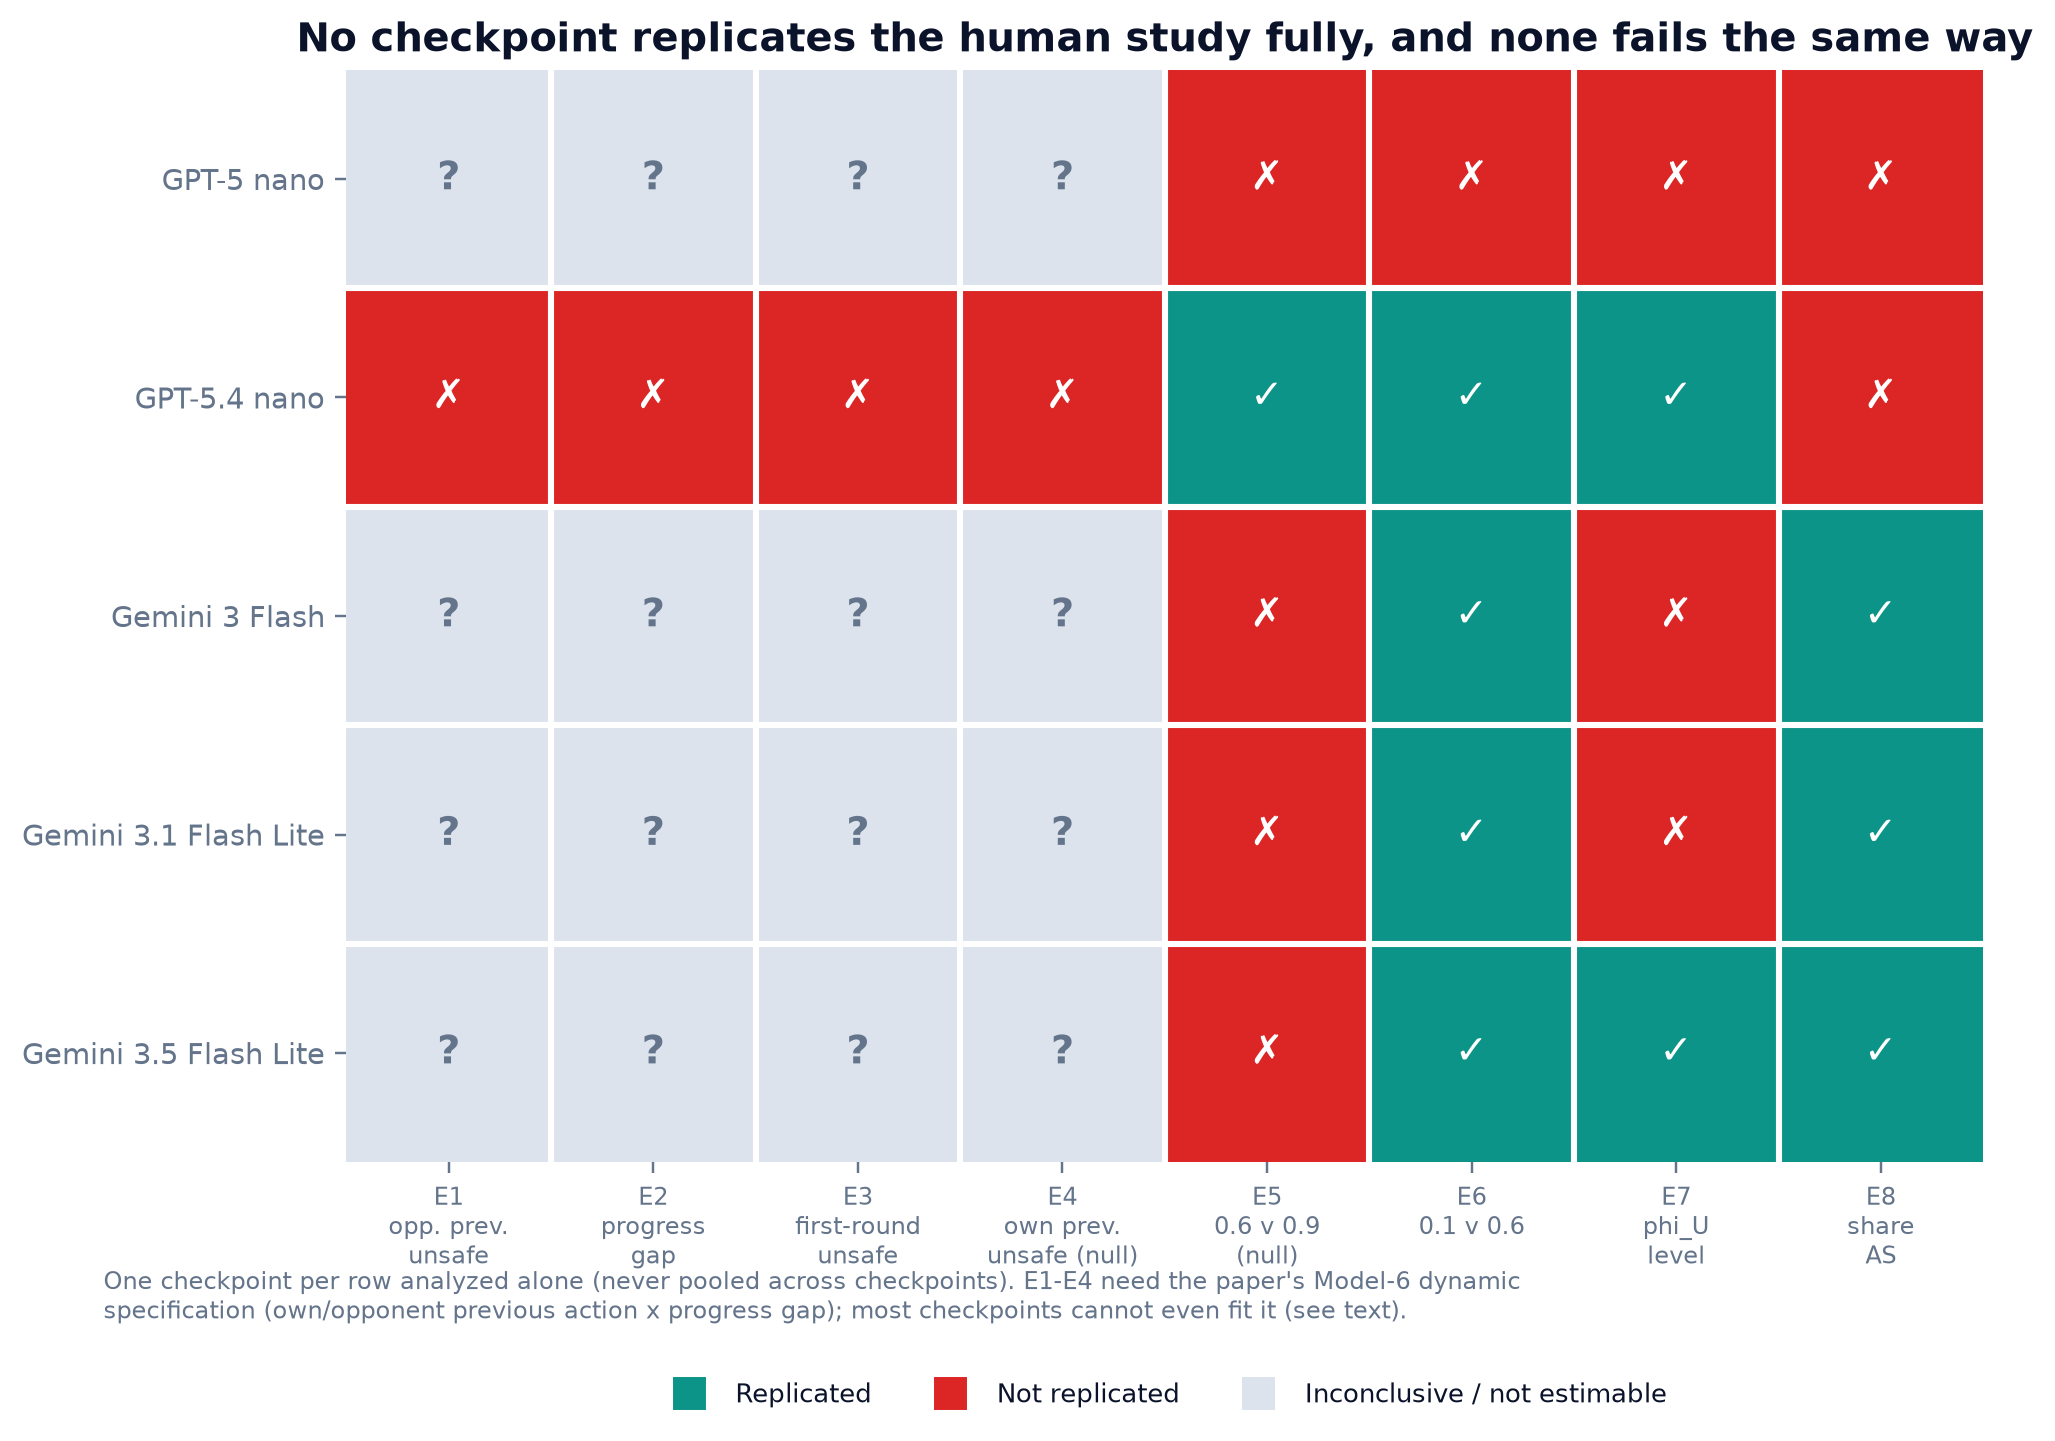
\includegraphics[width=.92\linewidth]{figures/human_effect_scorecard.png}
\caption{Cùng thông tin với Bảng~\ref{tab:scorecard}. Không mô hình nào tái tạo đủ tám dấu hiệu và không mô hình nào sai theo cùng một kiểu.}
\label{fig:scorecard}\end{figure}

\clearpage
\section{H2: Rủi ro trong luật chơi hay cách gán vai trò quan trọng hơn?}
\label{sec:persona}

\textbf{Giả thuyết H2.} Mức rủi ro thật trong luật chơi sẽ ảnh hưởng hành vi
mạnh hơn nhãn vai trò R1--R6. \textbf{Kết luận: dữ liệu đi ngược H2.} Nhãn vai
trò liên hệ với thay đổi lớn hơn nhiều so với thay đổi mức rủi ro.

Từ R1 đến R6, tỷ lệ Mạo hiểm tăng đơn điệu ở mọi mô hình được thử: GPT-5 nano
từ khoảng 2\% lên 52\%, GPT-5.4 nano từ 0,4\% lên 99\%, Gemini 3 Flash từ
33\% lên 95\%. Trong khi giữ cố định vai trò, thay mức rủi ro từ 0.1 đến 0.9
chỉ làm đổi vài điểm phần trăm trong lần kiểm tra nhiều người chơi.

\begin{figure}[H]\centering
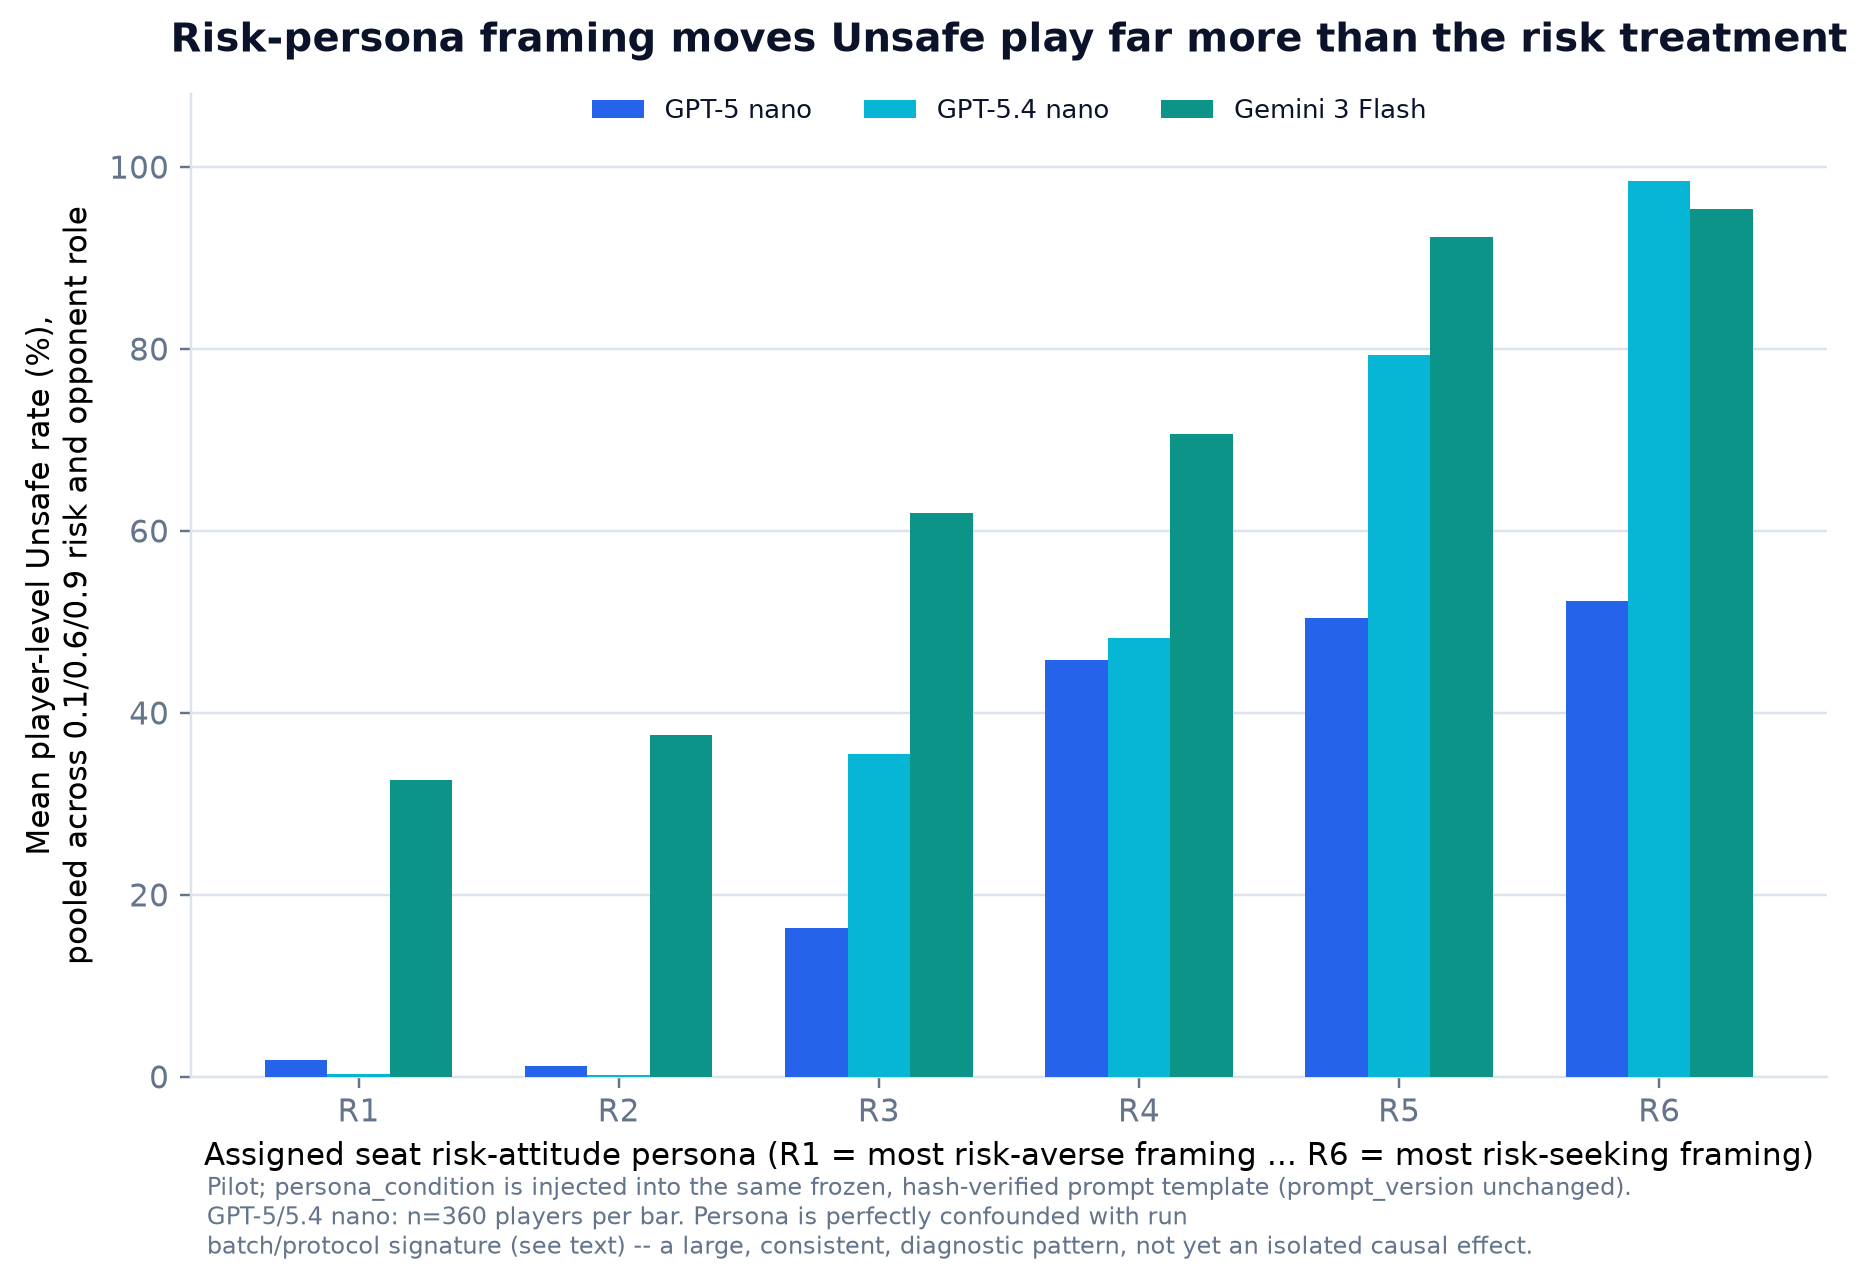
\includegraphics[width=.92\linewidth]{figures/persona_role_gradient.png}
\caption{Tỷ lệ Mạo hiểm theo vai trò của chính người chơi. R1 là khung mô tả thận trọng nhất; R6 là khung mô tả chấp nhận rủi ro nhất.}
\label{fig:persona-gradient}\end{figure}

\begin{luuy}[Giới hạn quan trọng]
Mỗi vai trò được chạy trong một lô riêng, nên không thể khẳng định chính nhãn
vai trò là nguyên nhân: hiệu ứng của lô chạy vẫn có thể lẫn vào. Câu trả lời
cần thiết là chạy các vai trò trong cùng một khối hạt ngẫu nhiên ở nghiên cứu
tiếp theo.
\end{luuy}

\clearpage
\section{H3: LLM có tái tạo các quy luật động của con người không?}
\label{sec:dynamic}

\textbf{Giả thuyết H3.} LLM sẽ phản ứng với lượt trước của đối thủ và với vị
thế dẫn/tụt giống con người. \textbf{Kết luận: phần lớn không tái tạo được.}
Chỉ một vài quy luật tổng quát giống nhau, còn mô hình hồi quy chi tiết thường
không ước lượng được hoặc cho hướng khác.

Trước hết, chúng tôi chạy lại mô hình của nghiên cứu gốc trên dữ liệu người.
Kết quả khớp gần như hoàn toàn: nếu đối thủ vừa chọn Mạo hiểm, hệ số là 0,606
($p=0,0016$); chênh lệch tiến độ của bản thân trừ đối thủ có hệ số $-0,295$
($p=0,048$). Hệ số âm ở đây có nghĩa là khi đang tụt hơn, con người có xu hướng
chọn Mạo hiểm hơn. Việc tái tạo này xác nhận cách xử lý dữ liệu.

Tuy nhiên, bốn trong năm mô hình không thể ước lượng ổn định cùng mô hình động:
một số gần như không bao giờ chọn Mạo hiểm ở lượt đầu, số khác gần như luôn
chọn Mạo hiểm. Khi một biến hầu như không thay đổi, dữ liệu không đủ thông tin
để ước lượng ảnh hưởng của nó. GPT-5.4 nano là ngoại lệ có thể ước lượng, nhưng
khoảng tin cậy cho phản ứng theo hành động trước của đối thủ ($-0,12$ đến 0,51)
vẫn chứa 0; ở người, khoảng này là 0,23 đến 0,99.

Điểm giống đáng chú ý: người thắng chọn Mạo hiểm nhiều hơn người thua, với chênh
lệch 16,0 điểm phần trăm ở người (64,3\% so với 48,3\%) và khoảng 20 điểm phần
trăm khi gộp mô tả năm LLM. Đây là tương quan với kết quả ván đấu, không chứng
minh Mạo hiểm gây ra chiến thắng.

Một khác biệt nền tảng bị che đi nếu chỉ nhìn trung bình: tỷ lệ Mạo hiểm của
từng người thật trải rộng gần hết khoảng 0--100\% và có nhiều cụm; mỗi mô hình
LLM lại nằm trong một dải hẹp riêng. Nghĩa là việc gọi lại cùng một mô hình đang
thay cho một chính sách khá ổn định, chứ không tái tạo được sự đa dạng giữa các
cá nhân người.

\begin{figure}[H]\centering
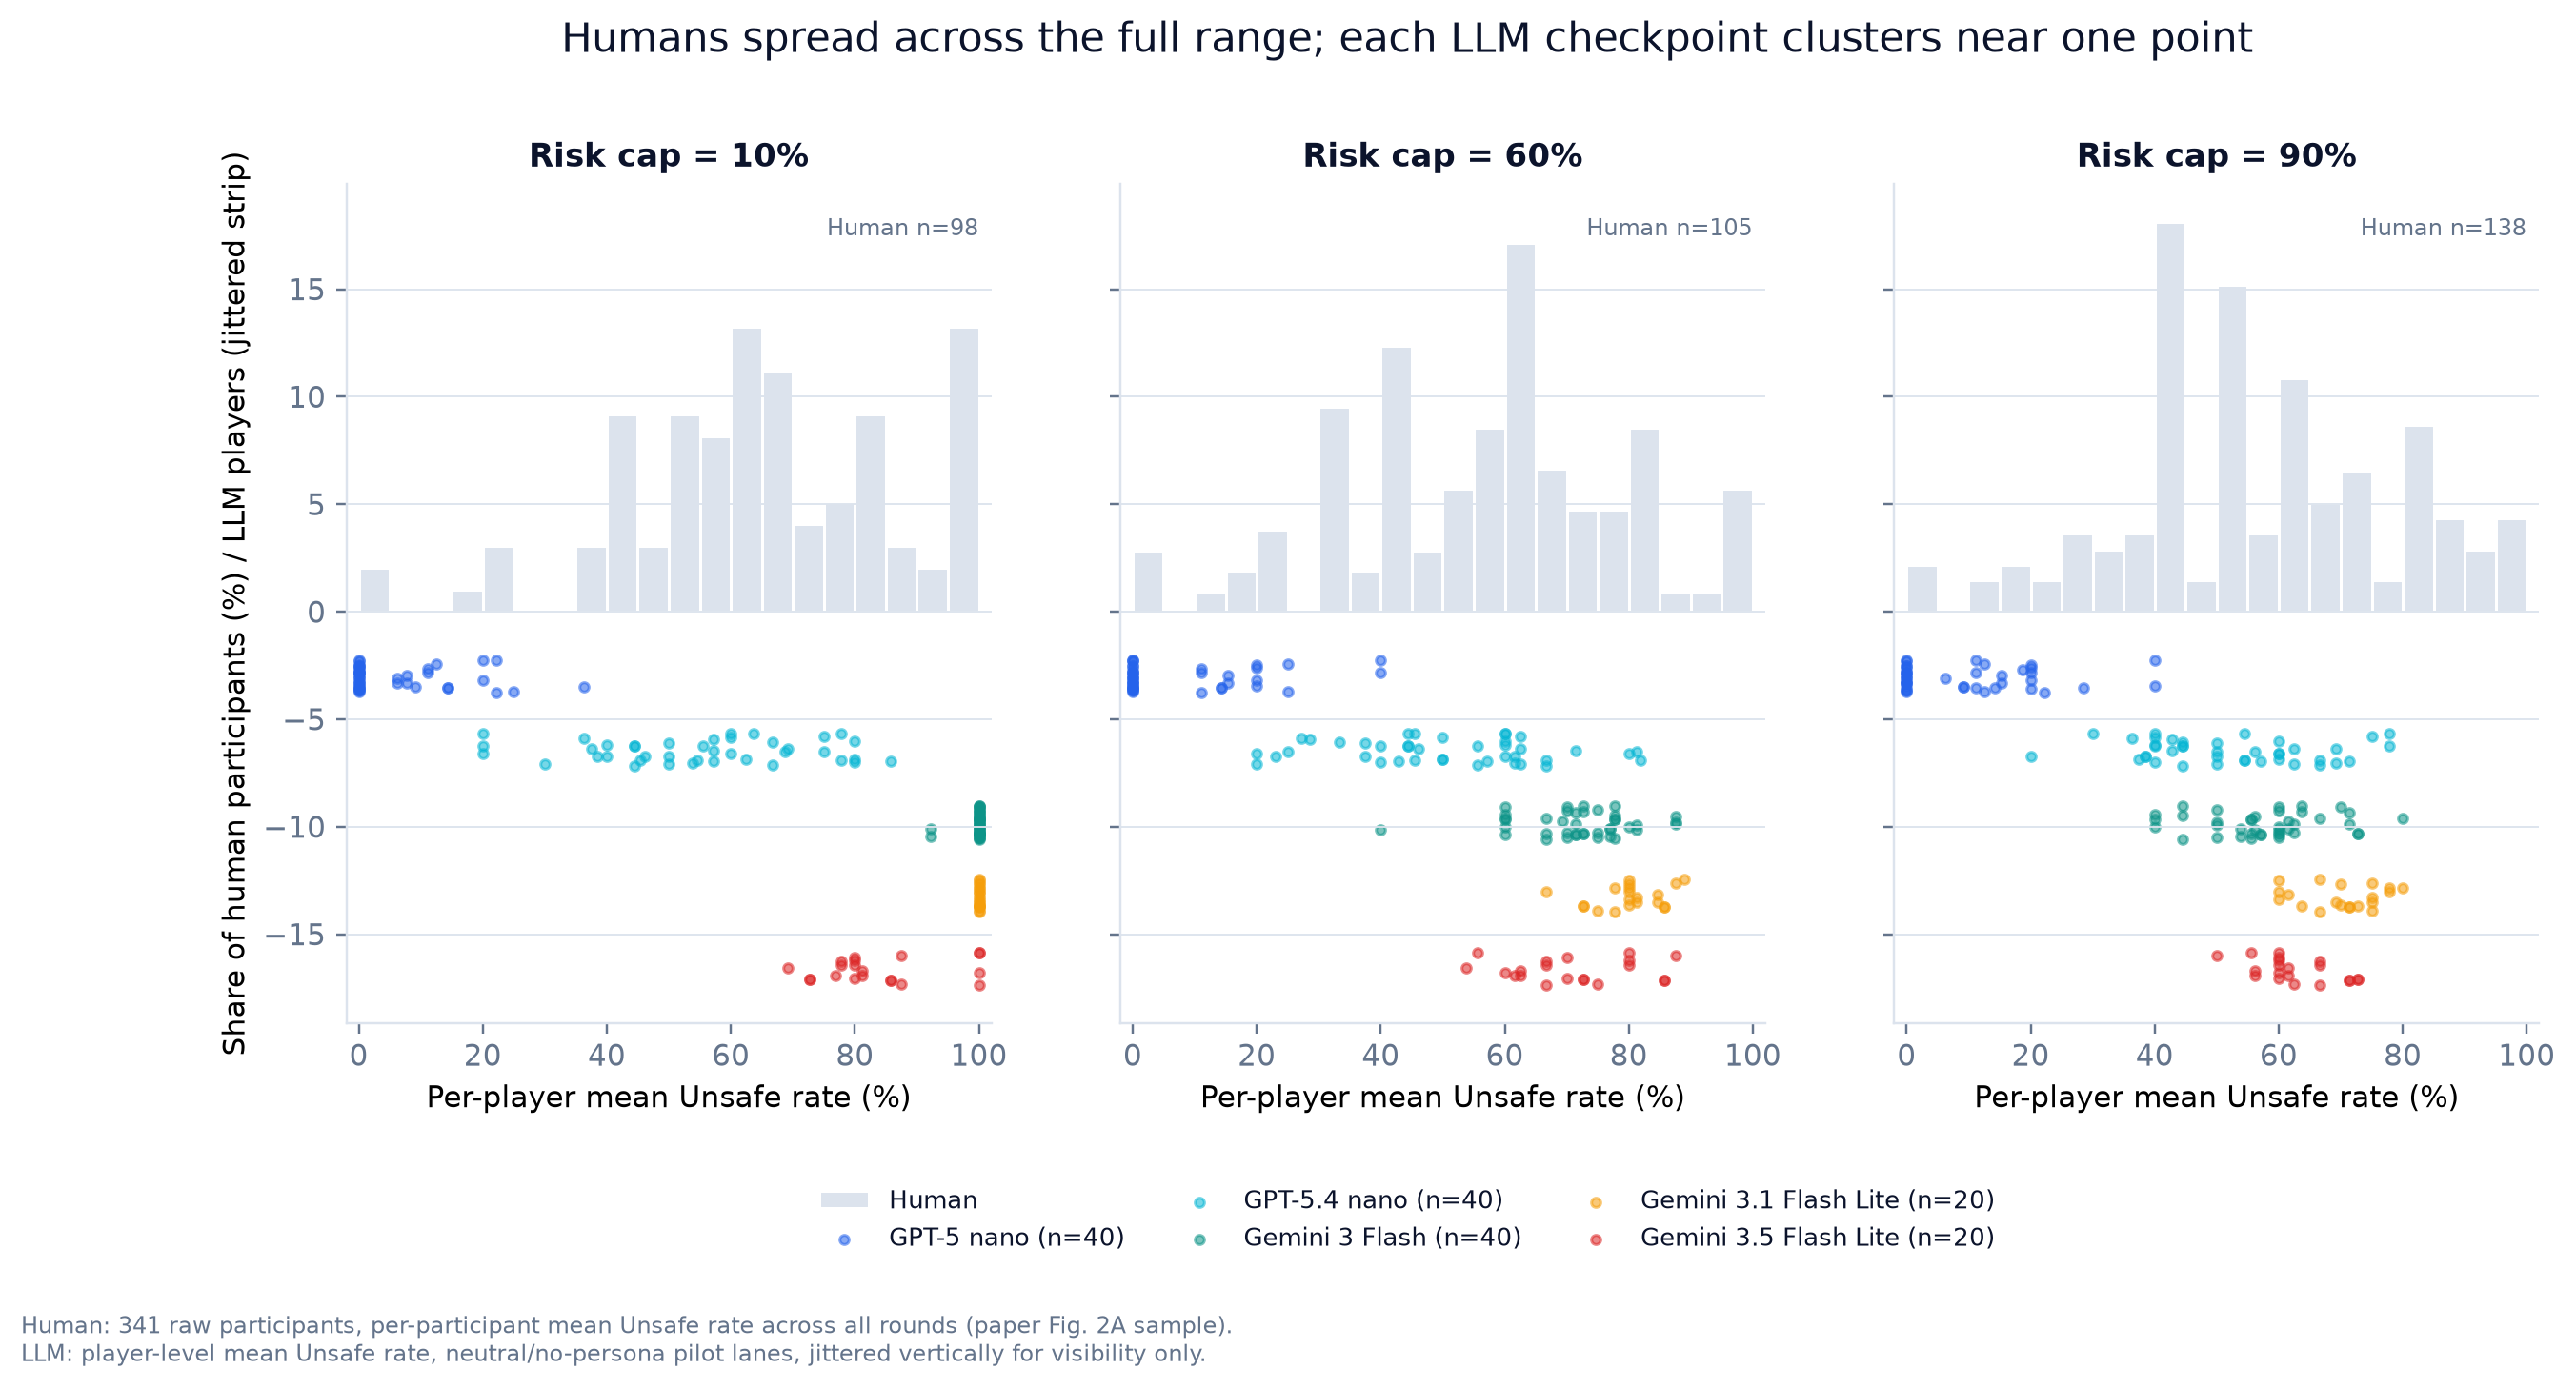
\includegraphics[width=.92\linewidth]{figures/human_vs_llm_distribution.png}
\caption{Phân bố tỷ lệ Mạo hiểm của từng người (màu xám) và từng lượt chơi của LLM (các điểm màu), theo mức rủi ro.}
\label{fig:distribution}\end{figure}

\begin{figure}[H]\centering

\includegraphics[width=.85\linewidth]{figures/human_vs_llm_dynamic_coefficients.png}
\caption{Hệ số các quy luật động ở người và GPT-5.4 nano, mô hình duy nhất có thể ước lượng đầy đủ. Thanh ngang là khoảng tin cậy 95\%.}
\label{fig:dynamic-coef}\end{figure}

\begin{luuy}[Một lỗi tài liệu của bộ dữ liệu công khai]
Biến \texttt{won\_race} được mô tả là không đổi trong toàn bộ các dòng của một
người, nhưng thực tế bằng 0 ở mọi lượt trừ lượt cuối. Phân tích dùng giá trị ở
lượt cuối cho toàn bộ ván. Điều này đã được báo ngược lại cho nguồn dữ liệu và
không ảnh hưởng việc tái tạo mô hình gốc.
\end{luuy}

\subsection{Diễn biến theo lượt}
Ở người, tỷ lệ Mạo hiểm giảm nhẹ từ lượt 1 (56,0\%) đến lượt 3 (51,3\%), tăng
lên đỉnh 62,6\% ở lượt 5, rồi dao động quanh 50--60\%. Không LLM nào lặp lại
gần hình dạng này. GPT-5 nano gần 0\% ở lượt 1, tăng vọt 22,5\% ở lượt 2 rồi
giảm. GPT-5.4 nano tăng từ 38,3\% lên khoảng 62,5\%. Các Gemini bắt đầu gần
100\%, giảm mạnh ở lượt 2, sau đó tăng lại. Mẫu này vẫn xuất hiện khi chỉ xét
các ván dài, nên không chỉ do các ván ngắn kết thúc sớm.

\clearpage
\section{H4: Những yếu tố dự báo lựa chọn có giống nhau không?}
\label{sec:feature-importance}

\textbf{Giả thuyết H4.} Các yếu tố quan trọng để dự báo lựa chọn Mạo hiểm sẽ
có thứ tự tương tự ở người và LLM. \textbf{Kết luận: bác bỏ H4.} Mỗi mô hình có
``dấu vân tay'' dự báo riêng.

Rừng ngẫu nhiên được học riêng cho từng nhóm từ năm thông tin có trước quyết
định: hành động trước của bản thân, hành động trước của đối thủ, chênh lệch
tiến độ, mức rủi ro và số lượt. Ở người, hành động trước của đối thủ chiếm
48\% độ quan trọng SHAP, lớn nhất. GPT-5 nano chủ yếu liên quan đến chênh lệch
tiến độ (44\%). Gemini 3 Flash và Gemini 3.1 Flash Lite chủ yếu liên quan đến
mức rủi ro (lần lượt 35\% và 40\%). Gemini 3.5 Flash Lite giống người nhất ở
khía cạnh này: hành động trước của đối thủ đứng đầu (34\%). GPT-5.4 nano không
có yếu tố nào áp đảo.

\begin{table}[H]\centering\small
\begin{tabular}{@{}lccccc@{}}\toprule
\textbf{Nhóm} & \textbf{Bản thân} & \textbf{Đối thủ} & \textbf{Chênh tiến độ} & \textbf{Rủi ro} & \textbf{Lượt}\\\midrule
Người & 6\% & \textbf{48\%} & 14\% & 12\% & 20\%\\
GPT-5 nano & 2\% & 4\% & \textbf{44\%} & 16\% & 33\%\\
GPT-5.4 nano & 18\% & 7\% & 33\% & 22\% & 20\%\\
Gemini 3 Flash & 5\% & 15\% & 23\% & \textbf{35\%} & 23\%\\
Gemini 3.1 Flash Lite & 16\% & 7\% & 13\% & \textbf{40\%} & 24\%\\
Gemini 3.5 Flash Lite & 14\% & \textbf{34\%} & 27\% & 17\% & 9\%\\
\bottomrule\end{tabular}
\caption{Tỷ trọng độ quan trọng SHAP. Mỗi hàng cộng thành 100\%; đây là mức độ hữu ích cho dự báo, không phải quan hệ nhân quả.}
\label{tab:shap}\end{table}

\begin{figure}[H]\centering
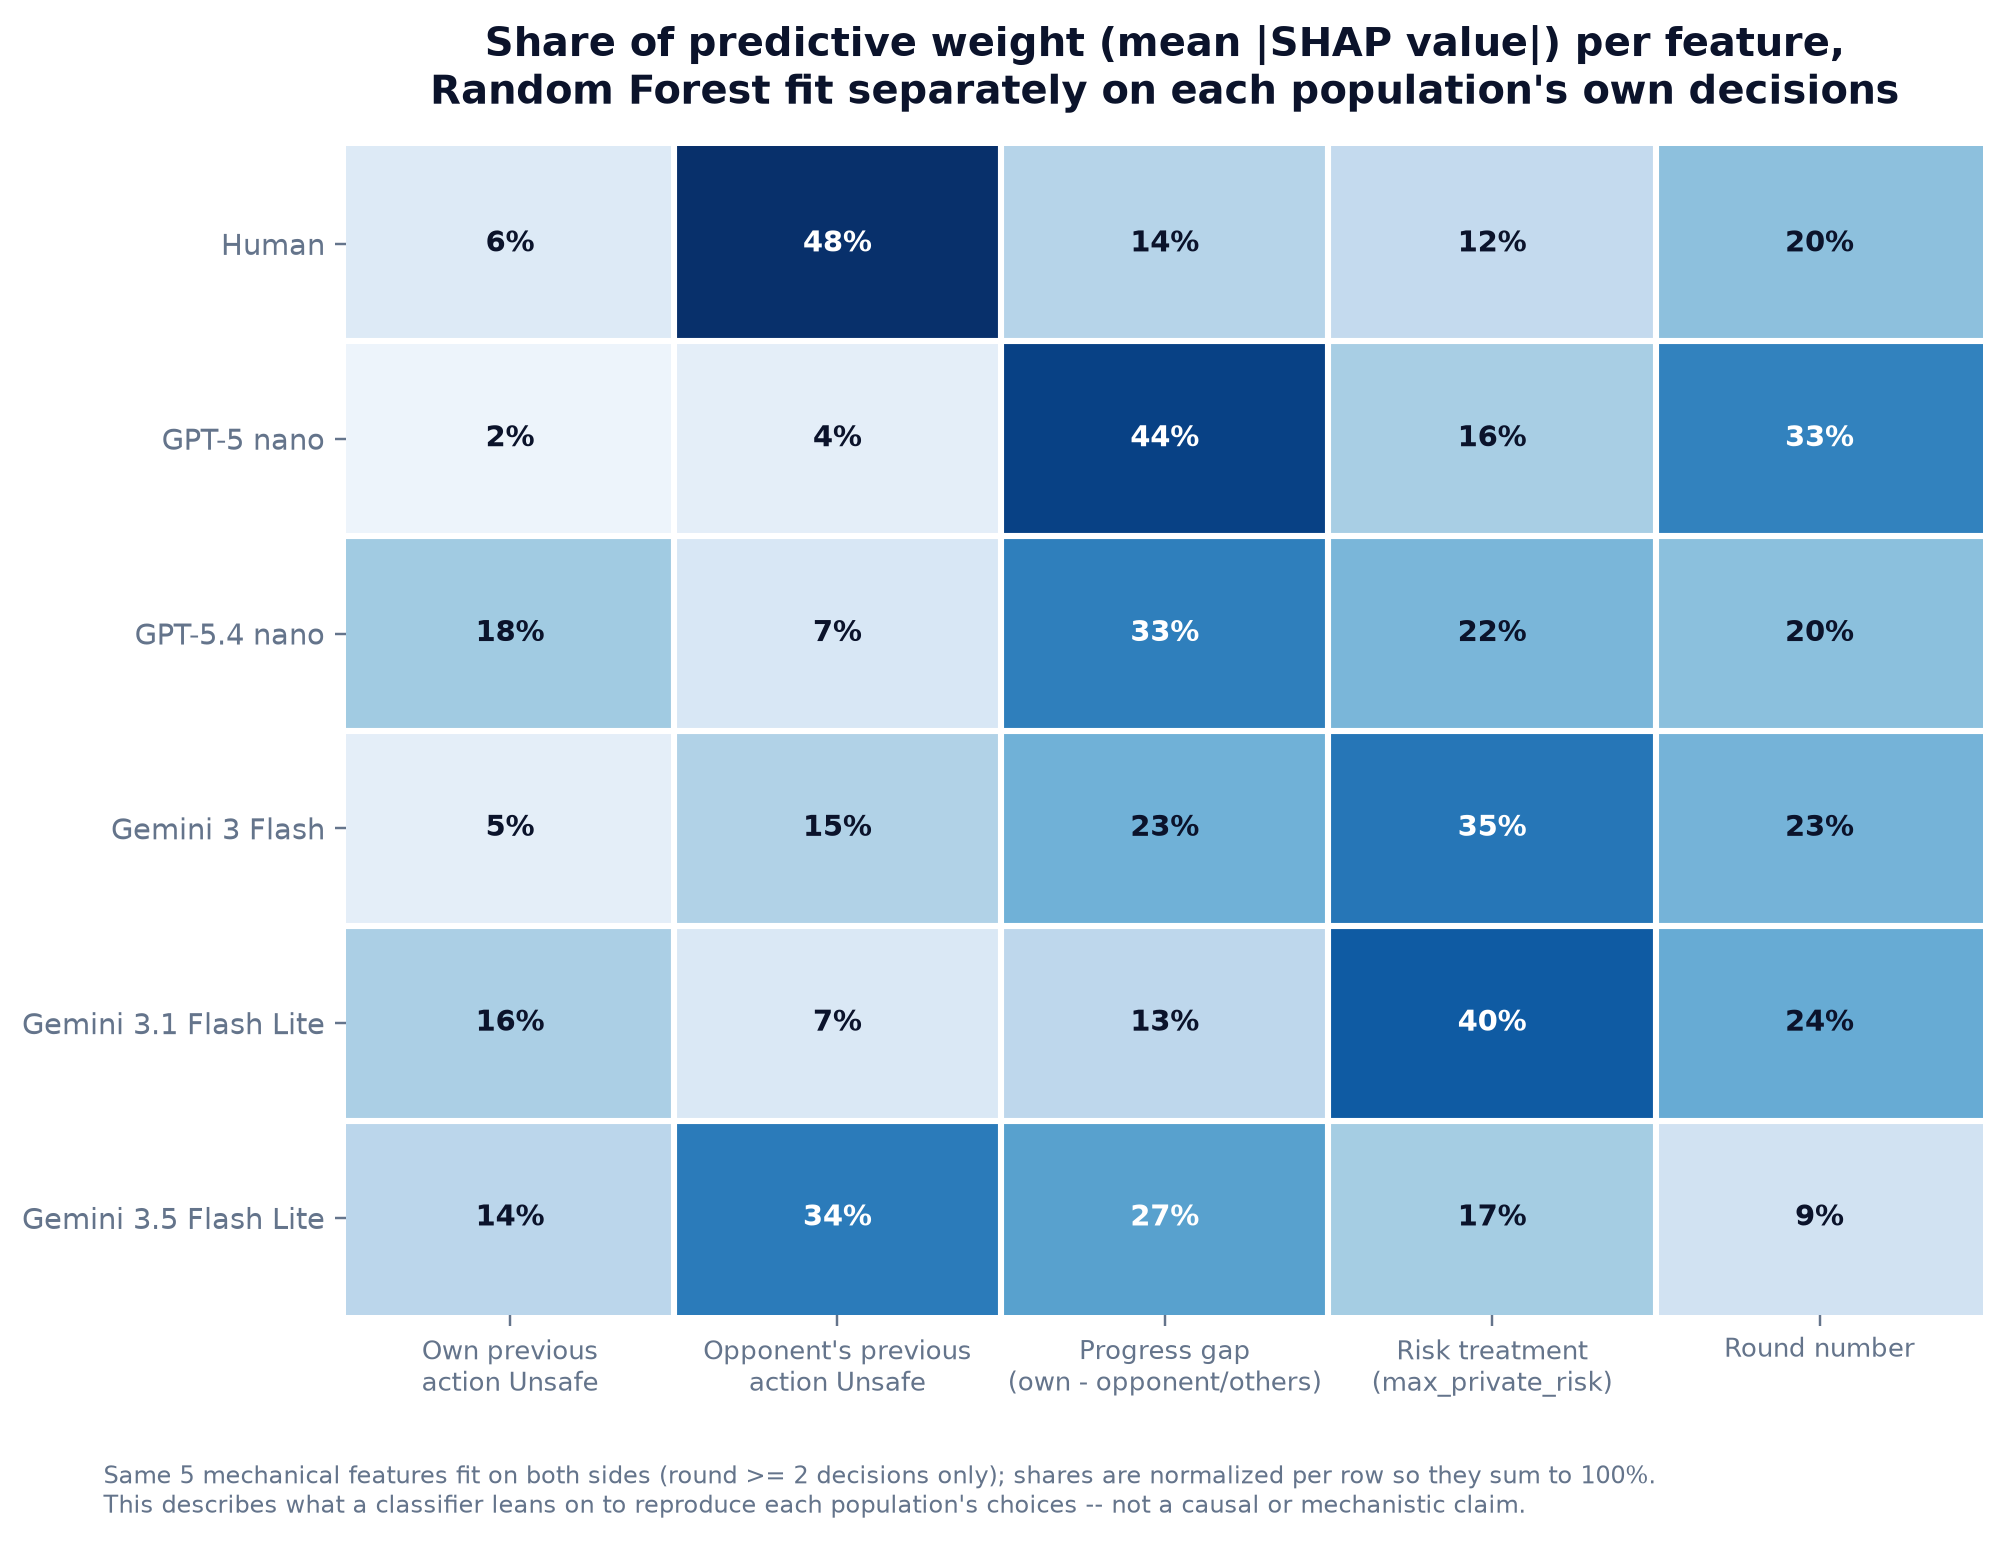
\includegraphics[width=.90\linewidth]{figures/feature_importance_shap_heatmap.png}
\caption{Biểu diễn trực quan Bảng~\ref{tab:shap}: mỗi hàng có một kiểu thông tin quan trọng khác nhau.}
\label{fig:shap}\end{figure}

\begin{luuy}
Độ chính xác dự báo thấp không có nghĩa một yếu tố không liên quan. Ví dụ, lựa
chọn của người khó dự báo bằng năm thông tin cơ học này, dù phản ứng với đối thủ
được ước lượng rõ. Các mô hình có tỷ lệ gần 0\% hoặc 100\% cũng làm chỉ số dự
báo bị méo.
\end{luuy}

Với dữ liệu người, thêm giới tính, tuổi, nhóm quốc tịch và kết quả bài đo sở
thích rủi ro trước trò chơi làm độ chính xác dự báo tăng từ 58,6\% lên 63,2\%.
Hành động trước của đối thủ vẫn quan trọng nhất (44\% theo SHAP), nhưng chỉ báo
Nam Phi (8,9\%) và tuổi (6,8\%) quan trọng hơn điểm bài đo sở thích rủi ro
(3,5\%). LLM không có biến tương ứng nên đây chỉ là kết quả cho người.

\clearpage
\section{H5: Tăng số người chơi có giữ nguyên kiểu hành vi không?}
\label{sec:nplayer}

\textbf{Giả thuyết H5.} Từ 2 sang 3--5 người chơi, các quy luật chính giữ
nguyên. \textbf{Kết luận: chỉ đúng một phần.} Vai trò vẫn rất quan trọng, nhưng
số người chơi và cách gán vai trò cho các thành viên khác có thể đổi dấu phản
ứng theo vị thế.

Ở trò chơi 3 người, khung ``đối đầu'' làm tỷ lệ Mạo hiểm cao hơn nhiều khung
``hợp tác'': GPT-5 nano 54,8\% so với 0,6\%; GPT-5.4 nano 90,4\% so với
21,2\%. Điều mới là, nếu bản thân đã mang khung đối đầu, càng nhiều đồng đội
cũng mang khung đối đầu thì hai mô hình lại Mạo hiểm \emph{ít hơn} một chút.
Người chơi mang khung hợp tác không cho thấy ảnh hưởng này.

Cụ thể, ở người chơi mang khung đối đầu, GPT-5 nano giảm từ 57,5\% xuống
50,9\% khi số đồng đội ``đối đầu'' tăng (Cohen's $d=0,37$, $p=0,013$); GPT-5.4
nano giảm từ 93,2\% xuống 89,7\% ($d=0,31$, $p=0,038$). Đây là hiệu ứng ``né
đối đầu'' nhỏ nhưng xuất hiện ở cả hai mô hình, trái với câu chuyện đơn giản
rằng nhiều người đối đầu hơn sẽ luôn kéo hành vi leo thang.

\begin{figure}[H]\centering

\includegraphics[width=.85\linewidth]{figures/nplayer_peer_composition_effect.png}
\caption{Tỷ lệ Mạo hiểm theo khung của bản thân và số đồng đội mang khung đối đầu, trong trò chơi 3 người.}
\label{fig:peer-composition}\end{figure}

Với GPT-5 nano, tăng nhóm từ 3 lên 4 hoặc 5 người đổi hẳn xu hướng lặp lại hành
động: ở 3 người, hệ số hành động trước của bản thân là $-1,92$ (có xu hướng đổi
hành động); ở 4 và 5 người, nó là $+0,65$ và $+0,60$ (có xu hướng lặp lại).

Kết quả H2 cũng lặp lại độc lập ở 3 người: độ chênh từ R1 đến R6 là 55,3 điểm
phần trăm với GPT-5 nano và 96,0 điểm với GPT-5.4 nano; ở trò chơi 2 người là
lần lượt 50,5 và 98,1 điểm. Tuy nhiên hình dạng không giống thí điểm Qwen trước
đó: GPT-5 nano tăng khá đều, còn GPT-5.4 nano có hai tầng rõ hơn.

\subsection{Phản ứng theo vị thế đổi dấu theo vai trò}
Chúng tôi xét ``vị thế'' là tiến độ của bản thân trừ tiến độ trung bình của
những người còn lại. Hệ số âm nghĩa là càng tụt càng Mạo hiểm; đây là hướng của
người. Trong trò chơi 3 người, ở R1--R2 hệ số của GPT-5 nano âm hoặc không ước
lượng được do mọi lựa chọn đều An toàn. Từ R4 đến R6, hệ số dương và có ý nghĩa:
đang dẫn lại đi kèm với Mạo hiểm nhiều hơn. GPT-5.4 nano cũng chuyển sang dương
từ R3--R4, khi dữ liệu còn đủ biến thiên để ước lượng.

\begin{table}[H]\centering\small
\begin{tabular}{@{}lcc@{}}\toprule
\textbf{Vai trò} & \textbf{GPT-5 nano} & \textbf{GPT-5.4 nano}\\\midrule
Không gán vai trò & $-0,084$ ($p=0,67$) & $+0,069$ ($p=0,72$)\\
R2 & \textbf{$-1,40$} ($p<0,001$) & Không ước lượng được\\
R3 & $+0,091$ ($p=0,45$) & \textbf{$+0,534$} ($p=0,006$)\\
R4 & \textbf{$+0,228$} ($p=0,013$) & \textbf{$+1,45$} ($p<0,001$)\\
R5 & \textbf{$+0,393$} ($p<0,001$) & Không ước lượng được\\
R6 & \textbf{$+0,303$} ($p<0,001$) & Không ước lượng được\\
\bottomrule\end{tabular}
\caption{Hệ số của vị thế lên xác suất chọn Mạo hiểm, trò chơi 3 người. ``Không ước lượng được'' thường do hành vi nằm sát 0\% hoặc 100\%.}
\label{tab:nplayer-position}\end{table}

\begin{figure}[H]\centering
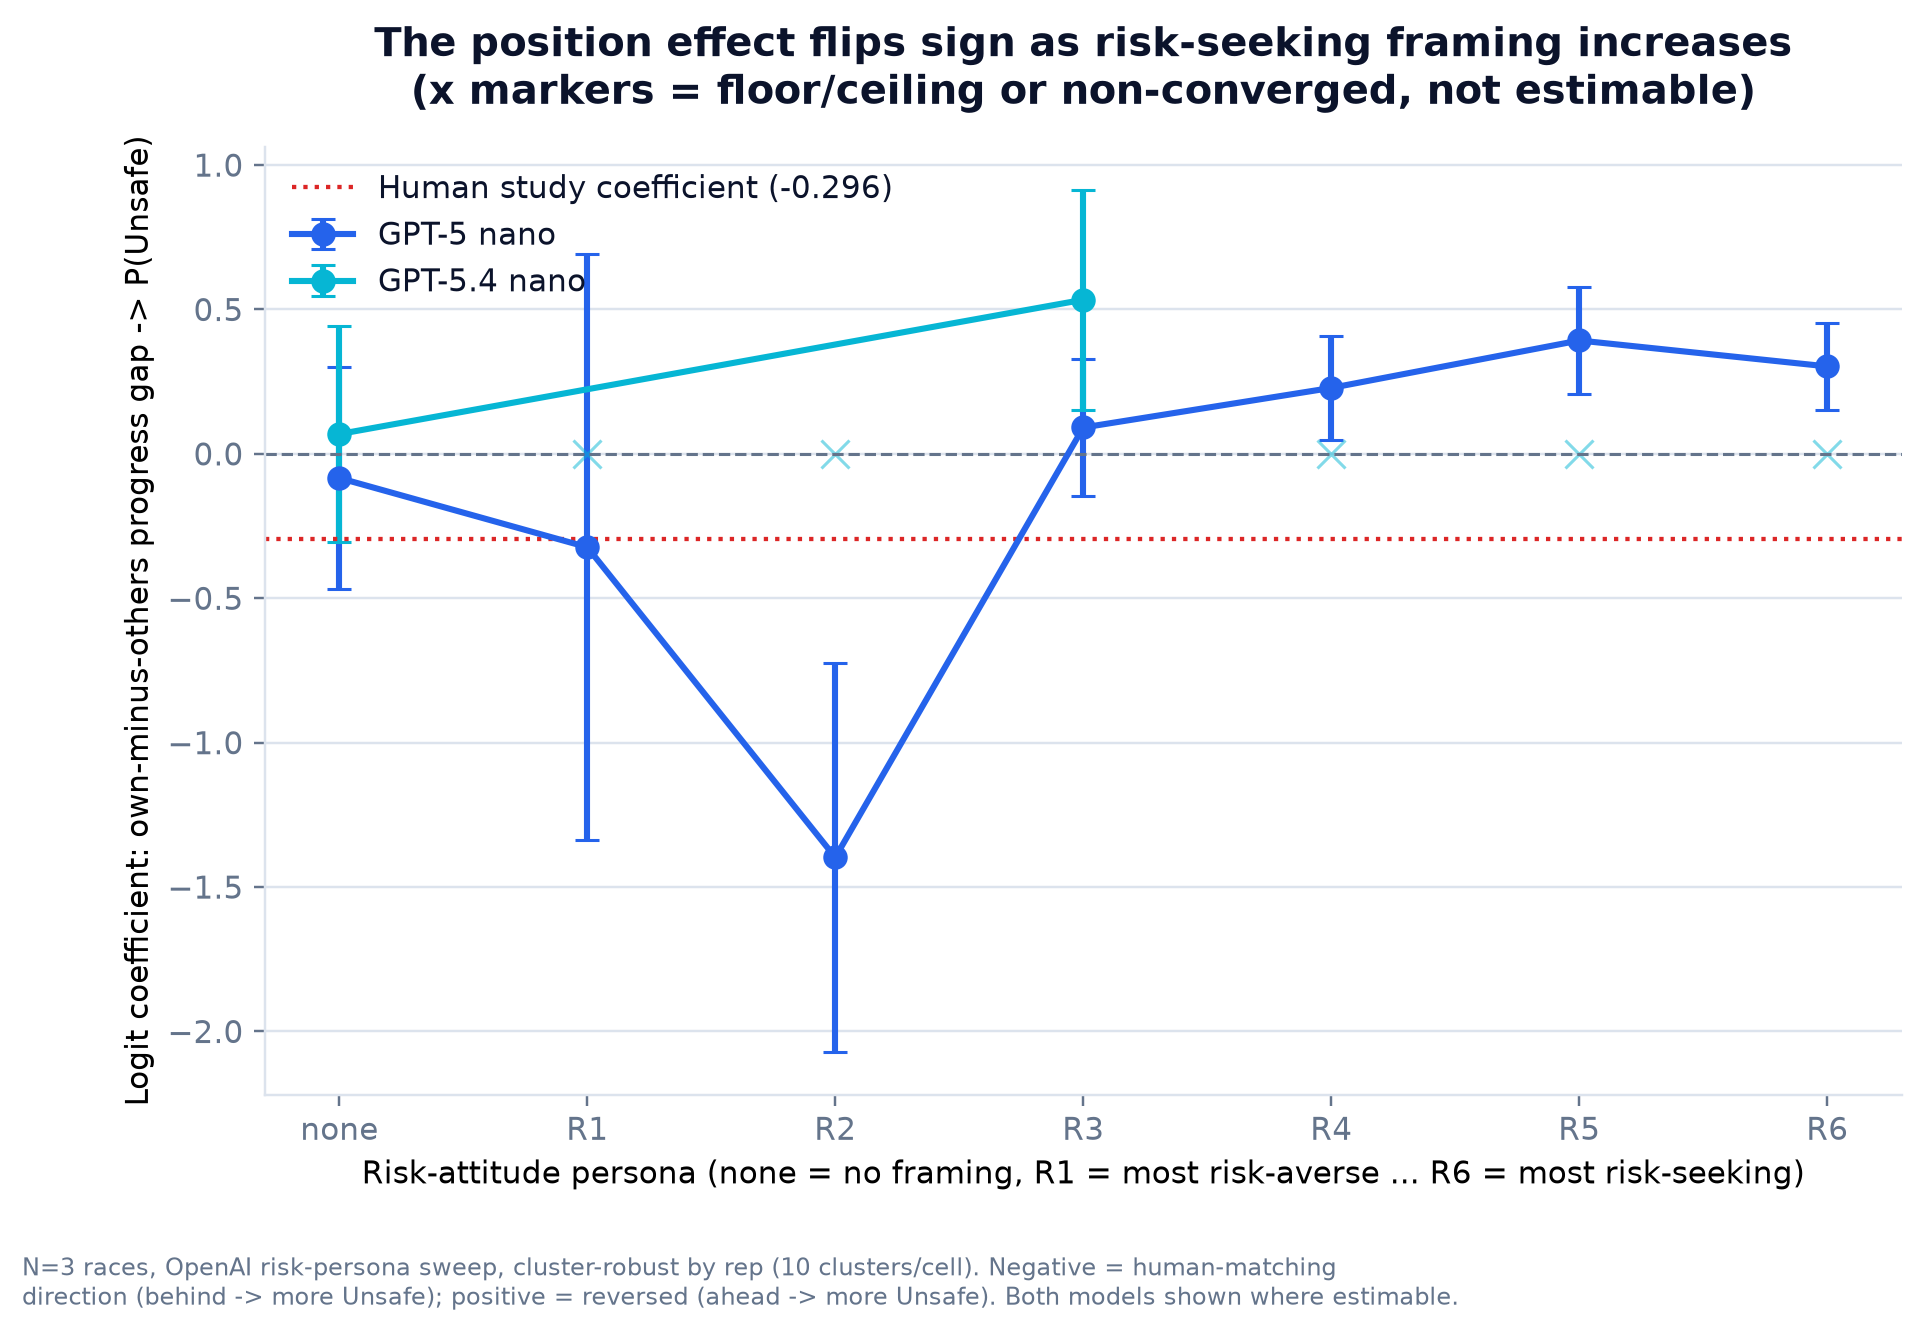
\includegraphics[width=.85\linewidth]{figures/nplayer_position_effect_sign_flip.png}
\caption{Hệ số vị thế theo vai trò trong trò chơi 3 người. Đường chấm đỏ là hướng của dữ liệu người.}
\label{fig:nplayer-position}\end{figure}

Đây là một kết quả cần kiểm tra lại, không phải cơ chế đã được chứng minh. Một
cách giải thích khả dĩ là vai trò thận trọng khiến người đang dẫn tiếp tục chơi
an toàn, còn vai trò chấp nhận rủi ro khiến người đang dẫn sẵn sàng tiếp tục
mạo hiểm. Với GPT-5.4 nano, xu hướng dương cũng xuất hiện ở trò chơi 2 người;
với GPT-5 nano, nó chỉ rõ ở trò chơi từ 3 người trở lên.

Đối chiếu trực tiếp trò chơi 2 người làm rõ điểm này. Với GPT-5.4 nano, hệ số
vị thế gần 0 ở điều kiện trung tính rồi dương rõ ở R3 ($+0,26$), R4 ($+0,23$)
và R5 ($+0,16$), tất cả $p<0,001$. Với GPT-5 nano, hệ số âm ở R3 ($-0,25$,
$p=0,001$) rồi nhỏ dần về 0 ở R4--R6, không chuyển sang dương. Vì vậy không
nên rút thành quy luật chung ``có vai trò chấp nhận rủi ro thì hiệu ứng luôn
đảo chiều''; nó còn tùy mô hình và số đối thủ.

\begin{figure}[H]\centering

\includegraphics[width=.85\linewidth]{figures/2p_position_effect_by_persona.png}
\caption{Bản đối chiếu của H5 cho trò chơi 2 người. GPT-5.4 nano đảo sang hệ số dương; GPT-5 nano chỉ tiến gần 0.}
\label{fig:2p-position}\end{figure}

\clearpage
\section{H6: Chọn Mạo hiểm nhiều hơn có luôn có lợi không?}
\label{sec:welfare}

\textbf{Giả thuyết H6.} Tỷ lệ Mạo hiểm cao hơn luôn đi với phần thưởng cuối
cùng cao hơn. \textbf{Kết luận: bác bỏ H6.} Kết quả phụ thuộc vào mô hình.

Với dữ liệu người, không có cột phần thưởng thực nhận. Chúng tôi chỉ tái dựng
được phần thưởng xấp xỉ từ điểm từng lượt và giải thưởng thắng ván; số này chưa
tính khoản mất do thụt lùi, nên chỉ là cận trên. Dữ liệu LLM có phần thưởng thực
nhận, gồm cả lần rút thăm thụt lùi.

\begin{table}[H]\centering\footnotesize
\begin{tabular}{@{}lccc@{}}\toprule
\textbf{Nhóm} & \textbf{Tương quan với thưởng xấp xỉ} & \textbf{Tương quan với thưởng thực} & \textbf{Tỷ lệ thụt lùi}\\\midrule
Người & $r=0,449$, $p<0,001$ & Không có dữ liệu & Không rõ\\
GPT-5 nano & $r=0,343$, $p<0,001$ & $r=-0,064$, $p=0,49$ & 4,2\%\\
GPT-5.4 nano & $r=0,754$, $p<0,001$ & $r=0,438$, $p<0,001$ & 21,7\%\\
Gemini 3 Flash & $r=0,246$, $p=0,007$ & $r=0,449$, $p<0,001$ & 34,2\%\\
Gemini 3.1 Flash Lite & $r=0,250$, $p=0,054$ & $r=0,428$, $p<0,001$ & 38,3\%\\
Gemini 3.5 Flash Lite & $r=0,203$, $p=0,12$ & $r=0,240$, $p=0,065$ & 31,7\%\\
\bottomrule\end{tabular}
\caption{Tương quan giữa tỷ lệ Mạo hiểm của từng người chơi và phần thưởng. Tương quan không cho biết Mạo hiểm là nguyên nhân của phần thưởng.}
\label{tab:welfare}\end{table}

Ở GPT-5 nano, lợi thế nhìn thấy khi bỏ qua thụt lùi biến mất hoàn toàn khi tính
phần thưởng thực. Ngược lại, GPT-5.4 nano vẫn có liên hệ dương rõ ràng. Với các
Gemini, liên hệ với phần thưởng thực còn mạnh hơn với thưởng xấp xỉ; có thể vì
những người Mạo hiểm nhiều cũng thường thắng ván, nhưng đây chỉ là diễn giải
khả dĩ chứ chưa phải kiểm định nhân quả.

\begin{figure}[H]\centering

\includegraphics[width=.92\linewidth]{figures/payoff_welfare_unsafe_vs_payoff.png}
\caption{Tỷ lệ Mạo hiểm và phần thưởng của từng người chơi. Dấu xám là thưởng xấp xỉ chưa tính thụt lùi; điểm màu là thưởng thực của LLM.}
\label{fig:welfare}\end{figure}

\clearpage
\section{H7: Gần dự đoán lý thuyết hơn có giống người hơn không?}

\textbf{Giả thuyết H7.} Mô hình có tỷ lệ Mạo hiểm gần dự đoán của lý thuyết trò
chơi tiến hóa hơn sẽ giống người hơn. \textbf{Kết luận: chưa đủ bằng chứng.}
Năm mô hình cho thấy các tương quan Pearson cùng hướng (từ $-0,41$ đến $-0,72$),
nhưng không có ý nghĩa thống kê; tương quan thứ hạng cũng không ổn định. Với
chỉ năm mô hình, không nên xem đây là một phát hiện.

Khoảng cách tuyệt đối trung bình với dự đoán lý thuyết của từng mô hình là:
GPT-5 nano 0,665; GPT-5.4 nano 0,403; Gemini 3 Flash 0,249; Gemini 3.1 Flash
Lite 0,258; Gemini 3.5 Flash Lite 0,323. Các tương quan Pearson với ba cách đo
``giống người'' (số dấu hiệu tái tạo được, tầm quan trọng của phản ứng với đối
thủ, và độ đa dạng các cụm hành vi) lần lượt là $-0,72$, $-0,41$ và $-0,49$;
nhưng kiểm định thứ hạng lần lượt là $-0,11$, $-0,62$, $-0,30$. Số mẫu $n=5$
quá nhỏ để suy luận đáng tin cậy.

Một đối chiếu nhỏ với quy trình giải thích mô hình trước đây cho Qwen cũng gợi ý
rằng mức rủi ro là thông tin hợp lệ quan trọng nhất, còn hành động trước của đối
thủ rất yếu. Thứ tự này gần các Gemini Lite hơn là con người. Tuy nhiên hai phân
tích dùng mô hình, điều kiện và phương pháp khác nhau, nên chỉ là tham chiếu
định hướng. Cụ thể, hai biến đứng đầu của quy trình Qwen cũ là thông tin lộ
đáp án (được tính gần như trực tiếp từ hành động vừa chọn) nên không được dùng
để diễn giải. Trong các biến hợp lệ có trước quyết định, mức rủi ro đứng thứ 10
trong khoảng 200 biến; số lượt thứ 37; hành động trước của bản thân thứ 43; còn
hành động trước của đối thủ thứ 130.

\clearpage
\section{Phân nhóm hành vi: kết quả bổ sung}
\label{sec:clustering}

Phân nhóm người chơi theo năm đặc điểm (tỷ lệ Mạo hiểm, phản ứng với đối thủ,
phản ứng khi dẫn/tụt, xu hướng lặp hành động, và lựa chọn lượt đầu) cho bốn nhóm
gần đúng: người khởi đầu thận trọng; người khởi đầu mạo hiểm và đáp trả đối thủ;
người mạo hiểm khi tụt và đáp trả mạnh; và nhóm nhỏ hay lặp hành động. Các nhóm
không tách biệt sắc nét, vì chỉ số phân tách ở mức yếu đến vừa (0,24--0,32).

Khi đặt các lượt chơi LLM vào cùng không gian của nhóm người, GPT-5 nano gần
như chỉ rơi vào nhóm khởi đầu thận trọng (99,2\%). Các Gemini chủ yếu rơi vào
hai nhóm khởi đầu mạo hiểm/đáp trả và mạo hiểm khi tụt. GPT-5.4 nano là mô hình
duy nhất chạm cả bốn nhóm. Điều này phù hợp với kết quả SHAP: GPT-5.4 nano không
bị một yếu tố duy nhất chi phối rõ.

\begin{table}[H]\centering\footnotesize
\begin{tabular}{@{}lcccc@{}}\toprule
\textbf{Mô hình} & \textbf{Khởi đầu thận trọng} & \textbf{Mạo hiểm/đáp trả} & \textbf{Đáp trả khi tụt} & \textbf{Hay lặp lại}\\\midrule
GPT-5 nano & \textbf{99,2\%} & 0\% & 0\% & 0,8\%\\
GPT-5.4 nano & 51,7\% & 33,3\% & 3,3\% & \textbf{11,7\%}\\
Gemini 3 Flash & 1,7\% & 78,3\% & 20,0\% & 0\%\\
Gemini 3.1 Flash Lite & 0\% & 83,3\% & 16,7\% & 0\%\\
Gemini 3.5 Flash Lite & 0\% & 76,7\% & 23,3\% & 0\%\\
\bottomrule\end{tabular}
\caption{Tỷ lệ mỗi mô hình gần nhất với từng cụm hành vi của người.}
\label{tab:cluster-projection}\end{table}

\begin{figure}[H]\centering

\includegraphics[width=.85\linewidth]{figures/llm_human_cluster_projection.png}
\caption{Cách các lượt chơi LLM được chiếu vào bốn cụm hành vi tạo từ dữ liệu người.}
\label{fig:cluster-projection}\end{figure}

Phân tích ban đầu tưởng như có nhiều người ``luân phiên'' An toàn--Mạo hiểm.
Sau khi hiệu chỉnh thiên lệch thống kê của chuỗi nhị phân ngắn bằng cách xáo
trộn từng chuỗi 2.000 lần, phần lớn dấu hiệu đó biến mất. Chỉ còn một nhóm rất
nhỏ ở người và một điều kiện vai trò của GPT-5 nano là ứng viên cho kiểu luân
phiên thực sự. Cụ thể, tỷ lệ ``luân phiên thật'' còn 25/303 người (8,3\%) và
126/1.329 lượt chơi LLM (9,5\%), gần mức 5\% có thể xuất hiện ngẫu nhiên. Ba ô
vai trò Gemini có dao động cao hơn, nhưng khớp tốt hơn với hai chiến lược đáp
trả đã có của dự án so với chiến lược tự lật hành động. Chỉ 25 người nói trên và
7/60 lượt ở ô GPT-5 nano đối đầu--hợp tác khớp tốt nhất với kiểu tự lật hành
động. Vì nhóm này rất nhỏ (7--25), nó chỉ là ứng viên cho chiến lược tham chiếu
thứ năm ở nghiên cứu xác nhận, không phải kết luận chính.

\section{Giới hạn}
\begin{itemize}[leftmargin=*]
\item Tất cả kết quả đều từ giai đoạn thí điểm; không dùng như kiểm định khẳng định.
\item Các hồi quy và độ quan trọng SHAP mô tả mối liên hệ trong dữ liệu, không xác định nguyên nhân.
\item Một số mô hình gần như luôn chọn một hành động, nên nhiều hệ số không thể ước lượng đáng tin cậy.
\item Xu hướng theo lượt có thể chịu ảnh hưởng vì các ván ngắn kết thúc sớm; kiểm tra chỉ với ván dài giảm nhưng không xóa hết lo ngại này.
\item Số liệu phần thưởng của người chỉ là ước tính cận trên vì thiếu biến cố thụt lùi thực tế.
\item Vai trò bị lẫn với lô chạy; cần thiết kế chạy xen kẽ vai trò trong cùng khối ngẫu nhiên để kiểm tra nhân quả.
\item Không gộp kết quả giữa mô hình, cấu trúc 2 người/nhiều người hay hai quần thể người--LLM.
\end{itemize}

\section{Kết luận}
Kết quả thí điểm không ủng hộ ý tưởng rằng có một kiểu hành vi chung cho ``LLM''
trong AI Race. Các mô hình khác nhau về phản ứng với rủi ro, thông tin nào chúng
dựa vào, diễn biến qua các lượt và việc Mạo hiểm có đi cùng phần thưởng thực hay
không. Phát hiện ổn định nhất là cách gán vai trò hoặc cách diễn đạt có liên hệ
với hành vi mạnh hơn thay đổi cơ học của mức rủi ro. Bước tiếp theo phù hợp là
nghiên cứu xác nhận với vai trò được ngẫu nhiên hóa trong cùng lô chạy, nhiều mô
hình hơn và tiêu chí đã đăng ký trước.

\end{document}
